\documentclass[../main.tex]{subfiles}
\begin{document}
\chapter{Programming in MATLAB}
\addcontentsline{toc}{section}{Chapter 4:Programming in MATLAB}

\section{SOME BASIC LOGIC}

Computers and their programs are designed to function very logically so that they always proceed by a well-defined set of rules. In order to write effective programs, we must first learn these rules so we can understand what a computer or MATLAB will do in different situations that may arise throughout the course of executing a program. The rules are set forth in the formal science of logic. Logic is actually an entire discipline that is considered to be part of both of the larger subjects of philosophy and mathematics. Thus there are whole courses (and even doctoral programs) in logic and any student who wishes to become adept in programming would do well to learn as much as possible about logic. Here in this introduction, we will touch only the surface of this subject, with the hope of supplying enough elements to give the student a working knowledge that will be useful in understanding and writing programs.\\

The basic element in logic is a \textbf{statement}, which is any declarative sentence or mathematical equation, inequality, etc. that has a \textbf{truth value} of either \textbf{true} or \textbf{false}.\\

\textbf{EXAMPLE 4.1:} For each of the English or mathematical expressions below, indicate which are statements, and for those that are, decide (if possible) the truth value.\\
(a) Al  Gore was Bill Clinton's Vice President\\
(b) $3<2$\\
(c) $x+3=5$\\
(d) If $x=6$ then $x^{2}>4 x$.\\

SOLUTION: All but (c) are statements. In (c), depending on the value of the variable $x$, the equation could be either true (if $x=2$ ) or false (if $x=$ any other number). The truth values of the other statements are as follows: (a) true, (b) false, and (d) true.

If you enter any mathematical relation (with one of the relational operators from Table 2.1), MATLAB will tell you if the statement is true or false in the following fashion:\\

\begin{tabular}{|l|l|}
\hline
Truth Value & MATLAB Code \\
\hline
True & 1 (as output) Any nonzero number (as input) \\
\hline
False & 0 (as input and output) \\
\hline
\end{tabular}


\begin{verbatim}
>>3<2
-> 0 (MATLAB is telling us the statement is false.)
>> x=6; x^2>4*x$
->1 (MATLAB is telling us the statement is true.)
\end{verbatim}

Logical statements can be combined into more complicated compound statements using \textbf{logical operators}. We introduce the four basic logical operators in Table 4.1, along with their approximate English translations, MATLAB code symbols, and precise meanings.\\

\textbf{TABLE 4.1}: The basic logical operators. In the meaning explanation, it is assumed the $p$ and $q$ represent statements whose truth values are known.

\begin{table}[H]
\resizebox{\textwidth}{!}{%
\begin{tabular}{@{}|l|l|l|l|l@{}}
\toprule
Name operator         & English Approximation & MATLAB Code & Meaning                                                                                                          &  \\ \midrule
Negation              & not p                 & $\sim$p     & $\sim$p is true if p is false, and false if p is true                                                            &  \\ \cmidrule(r){1-4}
Conjunction           & p and q               & p\&q        & p\&q is true if both p and q are ture, otherwise it's false.                                                     &  \\ \cmidrule(r){1-4}
Disjunction           & p or q                & p|q         & p|q is true in all cases except if p and q are both false,                                                       &  \\ \cmidrule(r){1-4}
Exclusive Disjunction & p or q (but not both)\footnotemark[1] & xor(p,q)    & xor(p,q) is true if exactly one of p or q is true. If p and q are both true or bothfalse then xor(p,q) is false. &  \\ \bottomrule
\end{tabular}%
}
\end{table}

\footnotetext[1]{Although most everyone understands the meaning of "and," in spoken English the word "or" is often
ambiguous. Sometimes it is intended as the disjunction but other times as the exclusive disjunction.
For example, if on a long airplane flight the flight attendant asks you, "Would you like chicken or
beef?" Certainly here the exclusive disjunction is intended—indeed, if you were hungry and tried to
ask for both, you would probably wind up with only one plus an unfriendly flight attendant. On the
other hand, if you were to ask a friend about his/her plans for the coming weekend, he/she might reply,
"Oh, I might go play some tennis or I may go to Janice's party on Saturday night." In this case the
ordinary disjunction is intended. You would not be at all surprised if your friend wound up doing both
activities In logic (and mathematics and computer programming) there is no room for such
ambiguity, so that is why we have two very precise versions of "or." }

\textbf{EXAMPLE 4.2}: Determine the truth value of each of the following compound statements.

(a) San Francisco is the capital of California and Egypt is in Africa.

(b) San Francisco is the capital of California or Egypt is in Africa.

(c) San Franciso is not the capital of California.

(d) not $(2>-4)$

(e) letting $x=2, z=6$, and $y=-4: x^{2}+y^{2}>z^{2} / 2$ or $z y<x$

(f) letting $x=2, z=6$, and $y=-4: x^{2}+y^{2}>z^{2} / 2$ or $z y<x$ (but not both)\\

SOLUTION: To abbreviate parts (a) through (c) we introduce the symbols:

$p=$ San Francisco is the capital of California.

$q=$ Egypt is in Africa.\\

From basic geography, Sacremento is California's capital so $p$ is false, and $q$ is certainly true. Statements (a) through (c) can be written as: $p$ and $q, p$ or $q$, not $p$, respectively. From what was summarized in Table $4.1$ we now see (a) is false, (b) is true, and (c) is true.

For part (d), since $2>-4$ is true, the negation not $(2>-4)$ must be false.

For parts (e) and (f), we note that substituting the values of $x, y$, and $z$ the statements become:

(e) $20>18$ or $-24<2$ i.e., true or true, so true

(f) $20>18$ or $-24<2$ (but not both), i.e., true or true (but not both), so false.\\

MATLAB does not know geography but it could have certainly helped us with the mathematical questions (d) through (f) above. Here is how one could do these on MATLAB:

\begin{verbatim}
>>~(2>-4)
-> 0 (=false)
>> x=2; z = 6; y=-4; (x^2+y^2 > z^2/2) | (z*y < x)
->1 (=true)
>>x=2; z=6; y=-4; xor(x^2+y^2 > z^2/2, z*x<x)
-> 0 (=false) 
\end{verbatim}

\hrule width \hsize \kern 1pt \hrule width \hsize height 0.4pt

\hspace{0.1cm}

\textbf{EXERCISES 4.1: }

\begin{enumerate}
\item For each of the English or mathematical expressions below, indicate which are statements, and for those that are statements, decide (if possible) the truth value.

(a) Ulysses Grant served as president of the United States.

(b) Who was Charlie Chaplin?

(c) With $x=2$ and $y=3$ we have $\sqrt{x^{2}+y^{2}}=x+y$.

(d) What is the population of the United States?

\item For each of the English or mathematical statements below, determine the truth value.

(a) George Harrison was a member of the Rolling Stones.

(b) Canada borders the United States or France is in the Pacific Ocean.

(c) With $x=2$ and $y=3$ we have $x^{x}>y$ or $x^{y}>y^{x}$.

(d) With $x=2$ and $y=3$ we have $x^{x}>y$ or $x^{y}>y^{x}$ (but not both).

\item Assume that we are in a MATLAB session in which the following variables have been stored: $x=6, y=12, z=-4$. What outputs would the following MATLAB commands produce? Of course, you should try to figure out these answers on your own and afterward use MATLAB to check your answers.

(a) $>>x+y>=z$

(b) $>>x \operatorname{xor}(z, x-2 * y)$

(c) $>>\left(x=-2 *z\right) \mid\left(x^{\wedge} 2>50  \&  y^{\wedge} 2>100\right)$

(d) $>>\left(x=2*z\right) \mid\left(x^{\wedge} 2>50 \& y^{\wedge} 2>100\right)$ 
\item The following while loops were separately entered in different MATLAB sessions. What will the resulting outputs be? Do this one carefully by hand and then use MATLAB to check your answers.

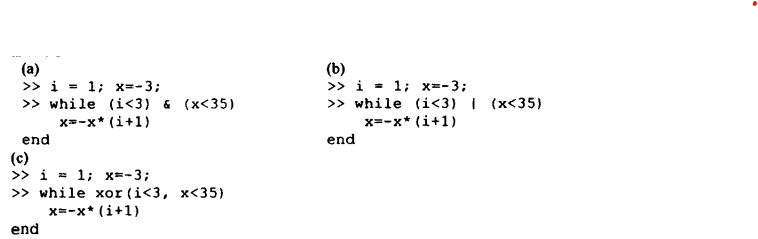
\includegraphics[max width=\textwidth]{code41}

\item The following while loops were separately entered in different MATLAB sessions. What will the resulting outputs be? Do this one carefully by hand and then use MATLAB to check your answers.\\

\begin{verbatim}
>>i = 1; x = 2; y = 3;
>> while (i<5) | (x==y)
	x = x*2,  y = y+x, i=i+1;
end
\end{verbatim}
\end{enumerate}

\section{LOGICAL CONTROL FLOW IN MATLAB}

Up to this point, the reader has been given a reasonable amount of exposure to while loops. The \emph{while loop} is quite universal and is particularly useful in those situations where it is not initially known how many iterations must be run in the loop. If we know ahead of time how many iterations we want to run through a certain recursion, it is more convenient to use a for loop. For loops are used to repeat (iterate) a statement or group of statements a specified number of times. The format is as follows:\\

\begin{figure}[H]
\centering
\begin{boxedverbatim}
>>for n=(start):(gap):(end )
	...MATLAB commands...
end
\end{boxedverbatim}
\end{figure}

The \textbf{counter} $n$ (which could be any variable of your choice) gets automatically bumped up at each iteration by the "gap." At each iteration, the "..MATLAB commands..." are all executed in order (just like they would be if they were to be entered manually again and again). This continues until the counter meets or exceeds the "end" number.

\begin{verbatim}
>> for n=1:5 \% if `gap` is ommited it is assumed to be 1. 
>> x(n) = n^3; \% we will be creating a vector of cubes of successive integers.
      end \% all output has been suppressed, but a vector x has been created
>> x \% let's display x now
-> x = 1 8 27 64 125
\end{verbatim}

Note that since a comma in MATLAB signifies a new line, we could also have
written the above for loop in a single line. We do this in the next loop below: \\

\begin{verbatim}
>> for n=1:2:10, x(k)=2; end
>> x \% we display x again. Try to guess what it now looks like.
-> x = 2 8 2 64 2 0 2 0 2 
\end{verbatim}

Observe that there are now nine entries in the vector $x$. This loop overwrote some of the five entries in the previous vector $x$ (which still remained in MATLAB's workspace). Let us carefully go through each iteration of this loop, explaining exactly what went on at each stage:
$k=1$ (start) $\rightarrow$ we redefine $x(1)$ to be 2 (from its original value of 1 ).
$k=1+2=3$ (augment $k$ by gap $=2) \rightarrow$ redefine $x(3)$ to be $2(x(2)$ was left to its original value of 8$)$.
$k=3+2=5 \rightarrow$ redefine $x(5)$ to be 2 .
$k=5+2=7 \rightarrow$ defines $\times(7)$ to be 2 (previously $x$ was a length 5 vector, now it has 7 components), the skipped component $x(6)$ is by default defined to be 0 . $k=7+2=9 \rightarrow$ defines $\times(9)$ to be 2 and the skipped $\times(8)$ to be 0 .
$k=9+2=11$ (exceeds end $=10$ so for loop is exited and thus completed).

The gap in a for loop can even be a negative number, as in the following example
that creates a vector in backwards order. The semicolon is omitted to help the
reader convince himself or herself how the loop progresses. 

\begin{verbatim}>> for i=3:-1: 1, y(i)=i, end\end{verbatim}
$\rightarrow y=0 \quad 0 \quad 3$

$\rightarrow y=\begin{array}{lll}-y & 2 & 3\end{array}$

$\rightarrow y=1 \quad 2 \quad 3$

A very useful tool in programming is the if-branch. In its basic form the syntax is as follows:

\begin{figure}[H]
\centering
\begin{boxedverbatim}
>>if <conditions>
	...MATLAB commands...
end
\end{boxedverbatim}
\end{figure}

The way such an if-branch works is that if the listed <condition >(which can be any MATLAB statement) is true (i.e., has a nonzero value), then all of the "...MATLAB commands..." listed are executed in order and upon completion the if-branch is then exited. If the <condition> is false then the "..MATLAB commands..." are ignored (i.e., they are bypassed) and the if-branch is immediately exited. As with loops in MATLAB, if-branches may be inserted within loops (or branches) to deal with particular situations that arise. Such loops/branches are said to be nested. Sometimes if-branches are used to "raise a flag" if a certain condition arises. The following MATLAB command is often useful for such tasks:\\

\begin{tabular}{|l|l|}
\hline fprintf('<any English / text phrase>') -> & Causes MATLAB to print: <any English phrase>. \\
\hline
\end{tabular}\\

Thus the output of the command fprintf('Have a nice day!') will simply be $\rightarrow$ Have a nice day! This command has a useful feature that allows one to print the values of variables that are currently stored within a text phrase. Here is how such a command would work: We assume that (previously in a MATLAB session) the values $w=2$ and $h=9$ have been calculated and stored and we enter:

\begin{verbatim}
>>fprintf('the width of the rectangle is \%d,the length is \%d.', w, h)
->the width of the rectangle is 2, the length is 9.»
\end{verbatim}

Note that within the "text" each occurrence of \% was replaced, in order, by the (current) values of the variables listed at the end. They were printed as integers (without decimals); if we wanted them printed as floating point numbers, we would use of in place of ofd. Also note that MATLAB unfortunately put the prompt >> at the end of the output rather than on the next line as it usually does. To prevent this, simply add (at the end of your text but before the single right quote) $\backslash$ r-which stands for "carriage return." This carriage return is also useful for splitting up longer groups of text within an fprintf.\\

Sometimes in a nested loop we will want to exit from within an inner loop and at
other times we will want exit from the mother loop (which is the outermost loop
inside of which all the other loops/branches are a part of) and thus halt all
operations relating to the mother loop. These two exits can be accomplished
using the following useful MATLAB commands: 
\\
$
\begin{array}{|l|l|}
\hline \begin{array}{l}
\text { break (anywhere within a } \\
\text { loop) } \rightarrow
\end{array} & \begin{array}{l}
\text { Causes immediate exit only from the single loop in which } \\
\text { break was typed. }
\end{array} \\
\hline \begin{array}{l}
\text { return (anywhere within a } \\
\text { nested loop) } \rightarrow
\end{array} & \begin{array}{l}
\text { Causes immediate exit from the mother loop, or within a } \\
\text { function M-file, immediate exit from M-file (whether or } \\
\text { not output has been assigned). }
\end{array} \\
\hline
\end{array}
$\\

The next example illustrates some of the preceding concepts and commands.

\textbf{EXAMPLE 4.4:}Carefully analyze the following two nested loops, decide what
exactly they cause MATLAB to do, and then predict the exact output. After you
do this, read on (or use MATLAB) to confirm your predictions. \\
(a) 
\begin{verbatim}
	for n=1:5
		for k=1:3
		 a=n+k
	  	 if a>=4, break, end
		end
	end 
\end{verbatim}

NOTE: We have inserted tabs to make the nested loops easier to distinguish.
Always make certain that each loop/branch is paired with its own end. \\

(b) 
\begin{verbatim}
for n=1:5
for k=1:3 
a=n+k
if a>=4
fprintf('We stop since a has reached the value %d \r', a)
return
end
end
end 
\end{verbatim}

SOLUTION: Part (a): Both nested loops consist of two loops. The mother loop in each is, as usual, the outermost loop (with counter $n$ ). The first loop begins with the mother loop setting the counter $n$ to be 1 , then immediately moves to the second loop and sets $k$ to be 1 ; now in the second loop a is assigned to be the value of $n+k=1+1=2$ and this is printed (since there is no semicolon). Since a $=2$ now, the "if-condition" is not satisfied so the if-branch is bypassed and we now iterate the $k$-loop by bumping up $k$ by 1 (= default gap). Note that the mother loop's $n$ will not get bumped up again until the secondary $k$-loop runs its course. So now with $k=2$, a is reassigned as $\mathrm{a}=n+k=1+2=3$ and printed, the ifbranch is again bypassed and $k$ gets bumped up to 3 (its ending value), $a$ is now reassigned as $a=n+k=1+3=4$ (and printed). The if-branch condition is now met, so the commands within it (in this case only a single "break" command) are run. So we will break out of the $k$-loop (which is actually redundant at this point since $k$ was at its ending value and the $k$-loop was about to end anyway). But we are still progressing within the mother $n$-loop. So now $n$ gets bumped up by 1 to be 2 and we start afresh the $k$-loop again with $k=1$. The variable a is now assigned as $\mathrm{a}=n+k=2+1=3$ (and printed), the if-branch is bypassed since the condition is not met and $k$ gets bumped up to be 2 . Next a gets reassigned as $\mathrm{a}=$ $n+k=2+2=4$, and printed. Now the if-branch condition is met so we exit the $k$-loop (this time prematurely) and $n$ now gets bumped up to be 3 . Next entering the $k$-loop with $k=1$, a gets set to be $n+k=3+1=4$, and printed, the "ifbranch condition" is immediately satisfied, and we exit the $k$-loop and n now gets bumped up to be 4. As in the last iteration, the $k$-loop will just reassign a to be 5 and print this, break and $n$ will go to 5 (its final value). In the final stage, a gets assigned as 6 , the if-branch breaks us out of the $k$-loop, and since $\mathrm{n}$ is at its ending value, the mother loop exits.
The actual output for part (a) is thus:

\begin{verbatim}-> a=2  a=3  a=4  a=3  a=4  a=4  a=5  a=6\end{verbatim}


Part (b): Apart from the fprintf command, the main difference here is the replacement of the break command with the return command. As soon as the if-branch condition is satisfied, the conditions within will be executed and the return will cause the whole nested loop to stop in its tracks. The output will be as follows:\\

\begin{verbatim} -> a=2 a=3 a=4 We stop since a has reached the value 4\end{verbatim}\\

EXERCISE FOR THE READER 4.1: Below are two nested loops. Carefully analyze each of them and try to predict resulting outputs and then use MATLAB to verify your predictions. For the second loop the output should be given in the default format short.

(a)
\begin{verbatim}
>>for i=1:5
	i
	if i>2, fprintf('test'), end
end
\end{verbatim}

(b)
\begin{verbatim}
>>for i=l:8, x(i)=0; end %initialize vector
>>for i=6:-2:2
	for j=1:i
		x(i)-x(i)+1/j;
	end
end
>>x
\end{verbatim}
The basic form of the if-branch as explained above allows one to have MATLAB
perform a list of commands in the event that one certain condition is fulfilled. In
its more advanced form, if-branches can be set up to perform different sets of
commands depending on which situation might arise. In the fullest possible form,
the syntax of an if-branch is as follows: 

\begin{figure}[H]
\centering
\begin{boxedverbatim}
>> if <condition_1>
...MATLAB commands 1...
elseif <condition_2>
...MATLAB commands _2...
elseif <condition_n> ,
...MATLAB
else
...MATLAB
end 
\end{boxedverbatim}
\end{figure}

There can be any number of else if cases (with subsequent MATLAB commands) and the final else is optional. Here is how such an if-branch would function: The first thing to happen is that $<$ condition\_ $1>$ gets tested. If it tests true (nonzero), then the "...MATLAB commands\_1..." are all executed in order, after which the if-branch is exited. If $<$ condition\_ $1>$ tests false (zero), then the ifbranch moves on to the next <condition\_ $2>$ (associated with the first elseif). If this condition tests true, then "...MATLAB commands\_ $2 . .$ " are executed and the if-branch is exited, otherwise it moves on to test the next <condition\_3>, and so on. If the final else is not present, then once the loop goes through testing all of the conditions, and if none were satisfied, the if-branch would exit without performing any tasks. If the else is present, then in such a situation the "...MATLAB commands..." after the else would be performed as a catch-all to all remaining situations not covered by the conditions listed above.\\

Our next example will illustrate the use of such an extended if-branch and will also bring forth a rather subtle but important point.\\

\textbf{EXAMPLE 4.5:} Create a function M-file for the mathematical function defined by the formula:

$$
y= \begin{cases}-x^{2}-4 x-2, & \text { if } x<-1 \\ |x|, & \text { if }|x| \leq 1, \\ 2-e^{\sqrt{x-1},} & \text { if } x>1\end{cases}
$$

then store this M-file and get MATLAB to plot this function on the interval $-4 \leq x \leq 4$.

SOLUTION: The M-file can be easily written using an if-branch. If we use the filename ex4\_5, here is one possible M-file:

\begin{verbatim}
function y = ex4_5(x)
if x<-1
	y = -x.^2-4*x-2;
elseif x>1
	y = 2-exp(sqrt(x-1));
else
	y=abs(x);
end
end 
\end{verbatim}

It is tempting to now obtain the desired plot using the usual command sequence:

\begin{verbatim}>>x=-4:.001:4 ; y=ex4_5(x); plot(x,y) \end{verbatim}

There is a subtle problem here, though. If we were to enter these commands, we would obtain the graph of (the last function in the formula) $y=|x|$ on the whole interval $[-4,4]$. Before we explain this and show how to resolve this problem, it would behoove the reader to try to decide what is causing this to happen and to figure out a way to fix this problem.

If we carefully go on to see what went wrong with the last attempt at a plot, we observe that since $x$ is a vector, the first condition $\mathrm{x}<-1$ in the if-branch now becomes a bit ambiguous. When asked about such a vector inequality, MATLAB will return a vector of the same size as $x$ that is made up of zeros and ones. In each slot, the vector is 1 if the corresponding component of $x$ satisfies the inequality $(x<-1)$ and 0 if it does not satisfy this inequality. Here is an example:

\begin{verbatim}
>>[2 -5 3 -2 -1] < -1 %causes MATLAB to test each of the 5 inequalities as true (1)
						% or false (0)
->0 1 0 1 0
\end{verbatim}

Here is what MATLAB did in the above attempt to plot our function. Since $x$ is a (large) vector, the first condition $\mathrm{x}<-1$ produced another vector as the same size as $x$ made up of (both) 0's and 1's. Since the vector was not all true ( 1 's), the condition as a whole was not satisfied so it moved on to the next condition $\mathrm{x}>$ 1 , which for the same reason was also not satisfied and so bypassed. This left us with the catch-all command $\mathrm{y}=\mathrm{abs}(\mathrm{x})$ for the whole vector $x$, which, needless to say, is not what we had intended.\\

So now how can we fix this problem? One simple fix would be to use a for loop to construct the $y$-coordinate vector using ex 4 \_ (x) with only scalar values for $x$.\\

Here is one such way to construct $y$ :\\

\begin{minipage}[t]{.6\linewidth}
\begin{verbatim}
>> size(x) %first we find out
» % the size of x
-> 1 	8001
» for n=1:8001 0
y(n)=ex4_5(x(n) ) ;
end
>> plot(x,y) %now we can
>>% get the desired plot 
\end{verbatim}

\end{minipage}
\hspace{0.02\linewidth}
\begin{minipage}[t]{.5\linewidth}
  \strut\vspace*{-\baselineskip}\newline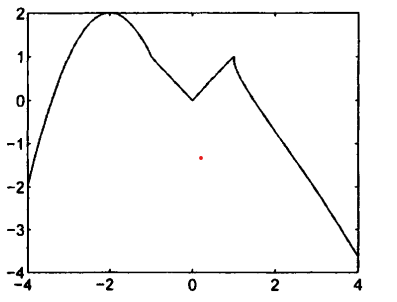
\includegraphics[width=\linewidth]{fig41}
  \captionof{figure}{The plot of the function of Example 4.5.  }
\label{fig:fig4_2}
\end{minipage}
 
  
A more satisfying solution would be to rebuild the M-file in such a way that when vectors are inputted for $x$, the if-branch testing is done separately for each component. The following program will do the job:

\begin{verbatim}
function y = ex4_5v2(x)
for i = 1:length(x)
if x(i)<-1
y(i) = -x(i).A
2-4*x(i)-2;
elseif x(i)>1
y(i) = 2-exp(sqrt(x(i)-1));
else
y(i)=abs(x(i) ) ;
end 
\end{verbatim}


With this M-file stored in our path the following commands would then indeed produce the desired plot of Figure 4.1:

\begin{verbatim}>> x=-4:.001:4 ; y=ex4_5v2(x); plot(x,y )\end{verbatim}

In dealing with questions involving integers, MATLAB has several numbertheoretic functions available. We mention three here. They will be useful in the
following exercise for the reader as well as in the exercises of this section. \\

$
\begin{array}{|l|l|}
\hline \begin{array}{l}
\text { floor(x)} \rightarrow
\end{array} & \begin{array}{l}
\text { Gives the greatest integer that is $\leq x$ (the \textbf{floor} of x). } \\
\end{array} \\
\hline \begin{array}{l}
\text { ceil(x)} \rightarrow
\end{array} & \begin{array}{l}
\text { Gives the least integer that is $\geq x$ (the \textbf{ceiling} of x). } \\
\end{array} \\
\hline \begin{array}{l}
\text { round(x)} \rightarrow
\end{array} & \begin{array}{l}
\text { Gives the nearest integer to x.  } \\
\end{array} \\
\hline
\end{array}
$ \\

For example, floor $(2.5)=2$, ceil $(2.5)=3$, ceil $(-2.5)=-1$, and round $(-2.2)=-2$. Observe that a real number $x$ is an integer exactly when it equals its floor (or ceiling, or round $(x)=x)$. EXERCISE FOR THE READER 4.2: (a) Write a MATLAB function M-file, call it sum2sq, that will take as input a positive integer $n$ and will produce the following output:\\

(i) In case $n$ cannot be written as a sum of squares (i.e., if it is not possible to write $n=a^{2}+b^{2}$ for some nonnegative integers $a$ and $b$ ) then the output should be the statement: "the integer $\langle n\rangle$ cannot be written as a sum of squares" (where $\langle n\rangle$ will print as an actual numerical value).

(ii) If $n$ can be written as a sum of squares (i.e., $n=a^{2}+b^{2}$ can be solved for nonnegative integers $a$ and $b$ ) then the output should be "the integer $\langle n\rangle$ can be written as the sum of the squares of $\langle a\rangle$ and $\langle b\rangle$ " (here again, $\langle n\rangle$ and also $\langle a\rangle$ and $\langle b\rangle$ will print as a actual numerical values) where $a$ and $b$ are actual solutions of the equation.

(b) Run your program with the following inputs: $n=5, n=25, n=12,233$, $n=100,000$.

(c) Write a MATLAB program that will determine the largest integer $<100,000$ that cannot be written as a sum of squares. What is this integer?

(d) Write a MATLAB program that will determine the first integer $>1000$ that cannot be written as a sum of squares. What is this integer?

(e) How many integers are there (strictly) between 1000 and 100,000 that cannot be expressed as a sum of the squares of two integers?

A useful MATLAB command syntax for writing interactive script M-files is the following:\\

$
\begin{array}{|l|l|}
\hline \begin{array}{l}
\text {$x=$ input ('<Enter input phrase>:      `)} \rightarrow
\end{array} & \begin{array}{l}
\text {When a script with this command is run, you will be } \\
\text {prompted in command window by the same  to enter}\\
\text {an input for script after which your input will} \\
\text {be stored as variable $x$ and the script will be executed.}
\end{array} \\
\hline
\end{array}
$ \\

The command can, of course, also be invoked in a function M-file, or at any time in the MATLAB command window. The next example presents a way to use this command in a nice mathematical experiment.

EXAMPLE 4.6: (Number Theory: The Collatz Problem) Suppose we start with any positive integer $a_{1}$, and perform the following recursion to define the rest of the sequence $a_{1}, a_{2}, a_{3}, \cdots$ :
$$
a_{n+1}=\left\{\begin{array}{ll}
a_{n} / 2, & \text { if } a_{n} \text { is even } \\
3 a_{n}+1, & \text { if } a_{n} \text { is odd }
\end{array} .\right.
$$

We note that if a term $a_{n}$ in this sequence ever reaches 1 , then from this point on the sequence will cycle through the values $1,4,2$. For example, if we start with $a_{1}=5$, the recursion formula gives $a_{2}=3 \cdot 5+1=16$, and then $a_{3}=16 / 2=8, a_{4}=8 / 2=4, a_{5}=4 / 2=2, a_{6}=2 / 2=1$, and so on $(4,2,1,4$, $2,1, \ldots)$. Back in 1937, German mathematician Lothar Collatz conjectured that no matter what positive integer we start with for $a_{1}$, the above recursively defined sequence will always reach the $1,4,2$ cycle. Collatz is an example of a mathematician who is more famous for a question he asked than for problems he solved or theorems he proved (although he did significant research in numerical differential equations). The Collatz conjecture remains an open problem to this day. \footnote[2]{The Collatz problem has an interesting history; see, for example [Lag-85] for some details. Many mathematicians have proved interesting results that strongly support the truth of the conjecture. For example, in 1972 , the famous Princeton number-theorist $\mathrm{J}$. H. Conway [Con-72] proved that if a Collatz iteration enters into a cycle other than $(1,4,2)$, the cycle must be of length at least 400 (i.e., the cycle itself must consist of at least 400 different numbers). Subsequently, J. C. Lagarias (in [Lag-85]) extended Conway's bound from 400 to 275,000 ! Recent high-speed computer experiments (in 1999 , by T. Oliveira e Silvio [OeS-99]) have shown the Collatz conjecture to be true for all initial values of the sequence less than about $2.7 \times 10^{16}$. Despite all of these breakthroughs, the problem remains unsolved. P. Erdós, who was undoubtedly one of the most powerful problem-solving mathematicians of the twentieth century, was quoted once as saying "Mathematics is not yet ready for such problems," when talking about the Collatz conjecture. In 1996 a prize reward of $£ 1,000$ (approx. $\$ 2,000$ ) was offered for settling the Collatz conjecture. Other math problems have (much) higher bounties. For example the Clay Foundation (URL: \href{http://www.claymath.org/prizeproblems/statement.htm}{www.claymath.org/prizeproblems/statement.htm}) has listed seven math problems and offered a prize of $\$ 1$ million for each one Enter a positive integer: 5 (MATLAB gives the first message, we only enter 5 , and enter to then get all of the informative output below.} Our next example will give a MATLAB script that is useful in examining the Collatz conjecture. Some of the exercises will outline other ways to use MATLAB to run some illuminating experiments on the Collatz conjecture.\\

\textbf{EXAMPLE 4.7:} We write a script (and save it as collatz) that does the following. It will ask for an input for a positive integer to be the initial value $a(1)$ of a Collatz experiment. The program will then run through the Collatz iteration scheme until the sequence reaches the value 1, and so begins to cycle (if ever). The script should output a sentence telling how many iterations were used for this Collatz experiment, and also give the sequence of numbers that were run through until reaching the value of 1.\\

\begin{verbatim}
%Collatz script
a(i) = input('Enter a positive integer: ') ;
n-1;
while a(n) ~= 1
if ceil(a(n)/2)==a(n)/2 %tests if a(n) is even
a(n+1)=a(n)/2;
else
a(n+1)=3*a(n)+l;
end
n=n1l;
end
fprintf('\r Collatz iteration with initial value a(1)= %d \r', a(D)
fprintf( took %d iterations before reaching the value 1 and ',n-1)
fprintf( beginning \r to cycle. The resulting pre-cycling')
fprintf(* sequence is as follows:')
a
clear a %lets us start with a fresh vector a on each run

Enter a positive integer: 5 (MATLAB gives the first message, we only enter 5, and enter to then get
all of the informative output below.)
-»Collate iteration with initial value a(1) = 5 took
5 iterations before reaching the value 1 and beginning
to cycle. The resulting pre-cycling sequence is as follows:
a =5 16 8 4 2 1 
\end{verbatim}\\


EXERCISE FOR THE READER 4.3: (a) Try to understand this script, enter it, and run it with these values: $a(1)=6,9,1,12,19,88,764$. Explain the purpose of the last command in the above script that cleared the vector a.\\

\hrule width \hsize \kern 1pt \hrule width \hsize height 0.4pt

\hspace{0.1cm}

\textbf{EXERCISES 4.2: }

\begin{enumerate}
\item Write a MATLAB function M-file, called sumodsq $(\mathrm{n})$, that does the following: The input is a positive integer $n$. Your function should compute the sum of the squares of all odd integers that do not exceed $n$ :
$$
1^{2}+3^{2}+5^{2}+\cdots+k^{2}
$$

where $k$ is the largest odd integer that does not exceed $n$. If this sum is less than I million, the output will be the actual sum (a number); if this sum is greater than or equal to 1 million, the output will be the statement " $<n>$ is too big" where $<n>$ will appear as the actual number that was inputted.

\item Write a function $\mathrm{M}$-file, call it sevenpow $(\mathrm{n})$, that inputs a positive integer $n$ and that figures out how many factors of $7 n$ has (call this number $k$ ) and outputs the statement: "The largest power of 7 which $\langle n\rangle$ contains as a factor is $\langle k\rangle . "$ So for example, if you run sevenpow(98) your output should be the sentence "The largest power of 7 which 98 contains as a factor is $2$." Run the commands: $sevenpow(36067)$, $sevenpow (671151153)$, and $sevenpow (3080641535629)$.
 
\item (a) Write a function M-file, call it sumsq $(n)$, that will input a positive integer $n$ and output the sum of the squares of all positive integers that are less than or equal to $n$ $(sumsq(n)$ $\left.=1^{2}+2^{2}+3^{2}+\cdots+n^{2}\right)$. Check and debug this program with the results $sumsq(1)=1$, $sumsq(3)=14$.

\item (a) Write a MATLAB function M-file, call it sum $2 s(n)$, that will take as input a positive integer $n$ and will produce for the output either of the following:

(i) The sum of all of the positive powers of $2(2+4+8+16+\ldots)$ that do not exceed $n$, provided this sum is less than 50 million.

(ii) In case the sum in (i) is greater than or equal to 50 million, the output should simply be "overflow""

(b) Run your function with the following inputs: $n=1, n=10, n=265, n=75,000$, $n=65,000,000$. 

(c) Write a short MATLAB code that will determine the largest integer $n$ for which this program does not produce "overflow."

\item (a) Write a MATLAB function M-file, called bigpro $(x)$, that does the following: The input is a real number $x$. The only output of your function should be the real number formed by the product $x(2 x)(3 x)(4 x) \cdots(n x)$, where $n$ is the first positive integer such that either $n x$ is an integer or $|n x|$ exceeds $x^{2}$ (whichever comes first).

(b) Of course, after you write the program you need to debug it. What values should result if we were to use the (correctly created) program to find: bigpro(4), bigpro(2.5), bigpro(12.7)? Run your program for these values as well as for the values $x=-3677 / 9, x=233.6461$, and $x=125,456.789$.

\item(\emph{Probability: The Birthday Problem}) This famous problem in probability goes as follows: If there is a room with a party of people and everyone announces his or her birthday, how many people (at least) would there need to be in the room so that there is more than a $50 \%$ chance that at least two people have the same birthday?
To solve this problem, we let $P(n)=$ the probability of a common birthday if there are $n$ people in the room. Of course $P(1)=0$ (no chance of two people having the same birthday if there is only one person in the room), and $P(n)=1$ when $n>365$ (there is a $100 \%$ chance, i.e., guaranteed, two people will have the same birthday if there are more people in the room than days of the year; we ignore leap-year birthdays). We can get an expression for $P(n)$ by calculating the complementary probability (i.e., the probability that there will not be a common birthday among $n$ different people). This must be
$$
\frac{365}{365} \cdot \frac{364}{365}, \frac{363}{365} \cdots \frac{366-n}{365}
$$
This can be seen as follows: The first person can have any of the 365 possible birthdays, the second person can have only 364 possibilities (since he/she cannot have the same birthday as the first person), the third person is now restricted to only 363 possible birthdays, and so on. We multiply the individual probabilities (fractions) to get the combined probability of no common birthday. Now this is the complementary probability of what we want (i.e., it must add to $P(n)$ to give $1=100 \%$ since it is guaranteed that either there is a common birthday or not). Thus
$$
P(n)=1-\frac{365}{365} \cdot \frac{364}{365} \cdot \frac{363}{365} \cdots \frac{366-n}{365}
$$
(a) Write a MATLAB function M-file for this function $P(n)$. Call the M-file bprob $(\mathrm{n})$ and set it up so that it does the following: If $n$ is a nonnegative integer, the function bprob (n) will output the sentence: "If a room contains $<n>$ people then the probability of a common birthday is $<P(n)>$ " where $<n>$ and $<P(n)>$ should be the actual numerical values. If $n$ is any other type of number (e.g., a negative number or 2.6) the output should be "Input $\langle n\rangle$ is not a natural number so the probability is undefined." Save your $M$-file and then run it for the following values: $n=3, n=6, n=15, n=90, n=110.5$, and $n=180$

(b) Write a MATLAB code that uses your function in part (a) to solve the birthday problem, i.e., determine the smallest $n$ for which $P(n)>.5$. More precisely, create a for loop whose only output will be: $n=$ the minimum number needed (for $P(n)$ to be $>.5$ ) and the associated probability $P(n)$.

(c) Get MATLAB to draw a neat plot of $P(n)$ vs. $n$ (for all $n$ between 1 and 365 ), and on the same plot, include the plots of the two horizontal lines with $y$-intercepts $.5$ and .9. Interpret the intersections.



\begin{minipage}[t]{.6\linewidth}
\item Write a function $M$-file, call it pythag $(n)$, that inputs a positive integer $n$ and determines whether $\boldsymbol{n}$ is the hypotenuse of a right triangle with sides of integer lengths. Thus your program will determine whether the equation $n^{2}=a^{2}+b^{2}$ has a solution with $a$ and $b$ both being positive integers.

\end{minipage}
\hspace{0.02\linewidth}
\begin{minipage}[t]{.5\linewidth}
  \strut\vspace*{-\baselineskip}\newline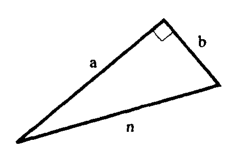
\includegraphics[width=\linewidth]{fig42}
  \captionof{figure}{Pythagorean triples. }
\label{fig:fig_4_2}
\end{minipage}

Such triples $n, a, b$ are called Pythagorean triples (Figure 4.2). In case there is no solution (as, for example, if $n=4$ ), your program should output the statement: "There are no Pythagorean triples with hypotenuse $\langle n\rangle$. " But if there is a solution your output should be a statement that actually gives a specific Pythagorean triple for your value of $n$. For example, if you type pythag $(5)$, your output should be something like: "There are Pythagorean triples having 5 as the hypotenuse, for example: $3,4,5$ is one such triple." Run this for several different values of $n$. Can you find a value of $n$ larger than 1000 that has a Pythagorean triple? Can you find an $n$ that has two different Pythagorean triples associated with it (of course not just by switching $a$ and $b$)?\\

HISTORICAL NOTE: Since the ancient times of Pythagoras, mathematicians have tried long and hard to find integer triple solutions of the corresponding equation with exponent $3: n^{3}=a^{3}+b^{3}$. No one has ever succeeded. In the 1700 s the amateur French mathematician Pierre Fermat conjectured that no such triples can exist. He claimed to have a truly remarkable proof of this but there was not enough space in the margin of his notes to include it. There has been an incredible amount of research trying to come up with this proof. Just recently, more than 300 years since Fermat stated his conjecture, Princeton mathematician Andrew Wiles came up with a proof. He was subsequently awarded the Fields medal, the most prestigious award in mathematics.

\item (\emph{Plane Geometry}) For an integer $n$ that is at least equal to 3 , a regular $n$-gon in the plane is the interior of a set whose boundary consists of $n$ flat edges (sides) each having the same length (and such that the interior angles made by adjacent edges are all equal). When $n=3$ we get an equilateral triangle, when $n=4$ we get a square, and when $n=8$ we get a regular octagon, which is the familiar stop-sign shape. There are regular $n$-gons for any such value of $n$; some are pictured in Figure 4.3.\\

\begin{figure}[H]

\includegraphics[max width=\textwidth]{fig43}
\caption{Some regular polygons}
\label{fig:fig_4_3}
\end{figure}

(a) Write a MATLAB function M-file, ngonper $1(n, d i a)$, that has two input variables, $n=$ the number of sides of the regular $n$-gon, and dia $=$ the diameter of the regular $n$-gons. The diameter of an $n$-gon is the length of the longest possible segment that can be drawn connecting two points on the boundary. When $n$ is even, the diameter segment cuts the $n$-gons into two congruent (equal) pieces. Assuming that $n$ is an even integer greater than 3 and dia is any positive number, your function should have a single output variable that equals the perimeter of the regular $n$-gons with diameter = dia. Your solution should include a handwritten mathematical derivation of the formula for this perimeter. This will be the hard part of this exercise, and it should be done, of course, before you write the program. Run your program for the following sets of input data: (i) $n=4$, dia $=\sqrt{4}$, (ii) $n=12$, dia $=12$, (iii) $n=1000$, dia $=5000$.

(b) Remove the restriction that $n$ is even from your program in part (a). The new function (call it now ngonper $(n$, dia) ) will now do everything that the one you constructed in part (a) did but it will be able to input and deal with any integer $n$ greater than or equal to 3 . Again, include with your solution a mathematical derivation of the perimeter formula you are using in your program. Run your program for these sets of values: (i) $n=3$, dia $=2$, (ii) $n=5$, dia $=4$, (iii) $n=999, \mathrm{dia}=500$.

(c) For which values of $n$ (if any) will your function in part (b) continue to give the correct perimeter of an $n$-gon that is no longer regular? An irregular $n$-gon is the interior of a set in the plane whose boundary consists of $n$ flat edges whose interior angles are not all equal. Examples of irregular $n$-gons include any nonequilateral triangle $(n=3)$, any quadrilateral that is not a square $(n=4)$. For those $n$ 's for which you say things still work, a (handwritten mathematical) proof should be included, and for those $n$ 's for which you say things no longer continue to work, a (handwritten) counterexample should be included.

\item (\emph{Plane Geometry}) This exercise consists of doing what is asked for in Exercise 8 (a)(b)(c) but with changing all occurrences of the word "perimeter" to "area." In parts (a) and (b) use the M-file names ngonar $1(n$, dia) and ngonarea ( $n$, dia).

\item (\emph{Finance: Compound Interest}) Write a script file called compints that will compute (as output) the future value $A$ in a savings account after prompting the user for the following inputs: the principal $P$ ( = amount deposited), the annual interest rate $r$ (as a decimal), the number $k$ of compoundings per year (so quarterly compounding means $k=4$, monthly means $k=12$, daily means $k=365$, etc.), and the time $t$ that the money is invested (measured in years). The relevant formula from finance is $A=P(1+r / k)^{k t}$. Run the script using the following sets of inputs: $P=\$ 10,000, r=8 \%(.08), k=4$, and $t=10$, then changing $t$ to 20 , then also changing $r$ to $11 \%$.

\textbf{Suggestion:} You probably want to have four separate "input" lines in your script file, the first asking for the principal, etc. Also, to get the printout to look nice, you should switch to format bank inside the script and then (at the very end) switch back to format short.

\item (\emph{Finance: Compound Interest}) Write a script file called comings that takes the same inputs as in the previous exercise, but instead of producing the output of the future account balance, it should produce a graph of the future value $A$ as a function of time as the time $t$ ranges from zero (day money was invested) until the end of the time period that was entered. Run the script for the three sets of data in the previous problem.

\item (\emph{Finance: Future Value Annuities}) Write a script file called fvanns that will compute (as output) the future value $F V$ in an annuity after prompting the user for the following inputs: the periodic payment $P M T$ (= amount deposited in account per period), the annual interest rate $r$ (as a decimal), the number $k$ of periods per year, that is, the number of compoundings per year (so quarterly compoundings/deposits means $k=4$, monthly means $k=12$, bimonthly means $k=24$, etc.), and the time $t$ that the money is invested (measured in years). The relevant formula from finance is $F V=P M T\left((1+r / k)^{k t}-1\right) /(r / k)$. Run the script using the following sets of inputs: $P M T=200, r=7 \%(.07), k=12$, and $t=30$, then changing $t$ to 40 , then also changing $r$ to $9 \%$. Next change $P M T$ to 400 on each of these three sets of inputs. Note, the first set of inputs could correspond to a worker who starts a supplemental retirement plan (say a $401(k)$ ), deposits $\$ 200$ each month starting at age 35 , and continues until he/she plans to retire at age $65(t=30$ years later). The $F V$ will be his/her retirement nest egg at time of retirement. The next set of data could correspond to the same retirement plan but started at age 25 ( 10 years more time). In each case compare the future value with the total amount of contributions. To encourage such supplemental retirement plans, the federal government allows such contributions (with limits) to be done before taxation.

\textbf{Suggestion:} You probably want to have four separate "input" lines in your script file, the first asking for the principal, etc. Also, to get the printout to look nice, you should switch to format bank inside the script and then (at the very end) switch back to format short.

\item (\emph{Finance: Future Value Anmuities}) In this exercise you will be writing a script file that will take the same inputs as in the previous exercise (interactively), but instead of just giving the future value at the end of the time period, this script will produce a graph of the growth of the annuity's value as a function of time.

(a) Base your script on the formula given in the preceding exercise for future value annuities. Call this script fvanngs. Run the script for the same sets of inputs that were given in the previous exercise.

(b) Rewrite the script file, this time constructing the vector of future values using a recursion formula rather than directly (as was asked in part (a)). Call this script fvanng2s. Run the script for the same sets of inputs that were given in the previous exercise.

\item (\emph{Number Theory: The Collatz Problem}) Write a function M-file, call it collctr, that takes as input, a positive integer an (the first element for a Collatz experiment), and has as output the positive integer $n$, which equals the number of iterations required for the Coliatz iteration to reach the value of 1 . What is the first positive integer $n$ for which this number of iterations exceegds 100? 200? 300?

\end{enumerate}

\section{WRITING GOOD PROGRAMS } %89
Up to this point we have introduced the two ways that programs can be written and stored for MATLAB to use (function M-files and script M-files) and we have also introduced the basic elements of control flow and a few very useful built-in MATLAB functions. To write a good program for a specified task, we will need to put all of our skills together to come up with an M-file that, above all, does what it is supposed to do, is efficient, and is as eloquent as possible. In this section we present some detailed suggestions on how to systematically arrive at such programs. Programming is an art and the reader should not expect to master it easily or in a short time.

STEP 1: Understand the problem, do some special cases by hand, and draw an outline. Before you begin to actually type out a program, you should have a firm understanding of what the problem is (that the program will try to solve) and know how to solve it by hand (in theory, at least). Computers are not creative. They can do very well what they are told, but you will need to tell them exactly what to do, so you had better understand how to do what needs to be done. You should do several cases by hand and record the answers. This data will be useful later when you test your program and debug it if necessary. Draw pictures (a flowchart), and write in plain English an explanation of the program, trying to be efficient and avoiding unnecessary tasks that will use up computer time.\\

STEP 2: Break up larger programs into smaller module programs. Larger programs can usually be split up into smaller independent programs. In this way the main program can be considerably reduced in size since it can call on the smaller module programs to perform secondary tasks. Such a strategy has numerous advantages. Smaller programs are easier to write (and debug) than larger ones and they may be used to create other large or improved programs later on down the road.\\

STEP 3: Test and debug every program. This is not an option. You should always test your programs with a variety of inputs (that you have collected output data for in Step 1) to make sure all of the branches and loops function appropriately. Novice and experienced programmers alike are often shocked at how rarely a program works after it is first written. It may take many attempts and changes to finally arrive at a fully functional program, but a lot of valuable experience can be gained in this step. It is one thing to look at a nice program and think one understands it well, but the true test of understanding programming is to be able to create and write good programs. Before saving your program for the first time, always make sure that every "for", "while", or "if" has a matching "end". One useful scheme when debugging is to temporarily remove all semicolons from the code, perhaps add in some auxiliary output to display, and then run your program on the special cases that you went through by hand in Step 1. You can see first-hand if things are proceeding along the lines that you intended.\\

STEP 4: \textbf {After it finally works, try to make the program as efficient and easy to read as possible.} Look carefully for redundant calculations. Also, try to find ways to perform certain required tasks that use minimal amounts of MATLAB's time. Put in plenty of comments that explain various elements of the program. While writing a complicated program, your mind becomes full of the crucial and delicate details. If you read the same program a few months (or years) later (say, to help you to write a program for a related task), you might find it very difficult to understand without a very time-consuming analysis. Comments you inserted at the time of writing can make such tasks easier and less time consuming. The same applies even more so for other individuals who may need to read and understand your program.\\

The efficiency mentioned in Step 4 will become a serious issue with certain problems whose programs (even good ones) will push the computer to its limits. We will come up with many examples of such problems this book. We mention here two useful tools in testing efficiency of programs or particular tasks. A flop (abbreviation for floating point operation) is roughly equivalent to a single addition, subtraction, multiplication, or division of two numbers in full MATLAB precision (rather than a faster addition of two single-digit integers, say). Counting flops is a common way of comparing and evaluating efficiency of various programs and parts thereof. MATLAB has convenient ways of counting flops \footnote[4]{ The flop commands in MATLAB are actually no longer available since Version 5 (until further notice). This is due to the fact that, starting with Version 6, the core programs in MATLAB got substantially revised to be much more efficient in performing matrix operations. It was unfortunate that the flop counting features could no longer be made to perform in this newer platform (collateral damage). Nonetheless, we will, on occasion, use this function in cases where flop counts will help to illustrate important points. Readers that do not have access to older versions of MATLAB will not be
able to mimic these calculations.} or elapsed time $(\mathrm{tic} / \mathrm{toc})$ :

$
\begin{array}{|l|l|}
\hline \begin{array}{l}
\text { flops(0) }\\
\text {...MATLAB commands...}\\
\text {flops }\\
\end{array} & \begin{array}{l}
\text { The flop s (0) resets the flop counter at zero. The flop s tells } \\
\text {the number of flops used to execute the "MATLAB commands" in}\\
\text {between. (Not available since Version 5, see Footnote 3.)} \\
\end{array} \\
\hline
\end{array}
$ \\


$
\begin{array}{|l|l|}
\hline \begin{array}{l}
\text {tic }\\
\text {...MATLAB commands...}\\
\text {toc }\\
\end{array} & \begin{array}{l}
\text {This tic resets the stopwatch to zero. The toe will tell the elapsed} \\
\text {time used The toe will tell the elapsed time used }\\
\text { to execute the "MATLAB commands.")} \\
\end{array} \\
\hline
\end{array}
$ \\

The results of $tic / toc$ depend not just on the MATLAB program but on the speed of the computer being used, as well as other factors, such as the number of other tasks concurrently being executed on the same computer. Thus the same MATLAB routines will take varying amounts of time on different computers (or even on the same computer under different circumstances). So, unlike flop comparisons, tic/toc comparisons cannot be absolute.\\

\textbf{EXAMPLE 4.8:} Use the tic/toc commands to compare two different ways of creating the following large vector: $[1 2 3  \cdots  10,000]$. First use the nonloop construction and then use a for loop. The results will be quite shocking, and since we will need to work with such large single vectors quite often, there will be an important lesson to be learned from this example. When creating large vectors in MATLAB, avoid, if possible, using "loops."

SOLUTION:

\begin{verbatim}
>>tic , for n=1:10000 , x(n)=n ; end, toc
->elapsed_time =8.9530 (time is measured in seconds)
>> tic , y=1:10000; toc
->elapsed_time = 0 
\end{verbatim}


This gives some basis for comparison. We see that the non-loop technique built a vector 10 times as large in about $1 / 1000$ of the time that it took the loop construction to build the smaller vector! The flop-counting comparison method would not apply here since no flops were done in these constructions.\\
 
Our next example will deal with a concept from linear algebra called the determinant of a square matrix, which is a certain important number associated with the matrix. We now give the definition of the determinant of a square $n \times n$ matrix \footnote[4]{The way we define the determinant here is different from what is usually presented as the definition. One can find the formal definition in books on linear algebra such as [HoKu-71]. What we use as our definition is often called \emph{cofactor expansion on the first row.} See [HoKu-71] for a proof that this is equivalent to the formal definition. The latter is actually more complicated and harder to compute and this is why we chose cofactor expansion}

$$
A=\left[\begin{array}{ccccc}
a_{11} & a_{12} & a_{13} & \cdots & a_{1 n} \\
a_{21} & a_{22} & a_{23} & \cdots & a_{2 n} \\
a_{31} & a_{32} & a_{33} & \ldots & a_{3 n} \\
\vdots & \vdots & \vdots & \ddots & \vdots \\
& & & & \\
a_{n 1} & a_{n 2} & a_{n 3} & \ldots & a_{n n}
\end{array}\right] \text {. }
$$
If $n=1$, so $A=\left[a_{11}\right]$, then the determinant of $A$ is simply the number $a_{11}$. If $n=2$, so $A=\left[\begin{array}{ll}a_{11} & a_{12} \\ a_{21} & a_{22}\end{array}\right]$, the determinant of $A$ is defined to be the number $a_{11} a_{22}-a_{12} a_{21}$ that is just the product of the main diagonal entries (top left to bottom right) less the product of the off diagonal entries (top right to bottom left).

For $n=3, \quad A=\left[\begin{array}{lll}a_{11} & a_{12} & a_{13} \\ a_{21} & a_{22} & a_{23} \\ a_{31} & a_{32} & a_{33}\end{array}\right]$ and the determinant can be defined using the $n=2$ definition by the so-called cofactor expansion (on the first row). For any entry $a_{i j}$ of the $3 \times 3$ matrix $A$, we define the corresponding submatrix $A_{i j}$ to be the $2 \times 2$ matrix obtained from $A$ by deleting the row and column of $A$ that contain the entry $a_{i j}$. Thus, for example,

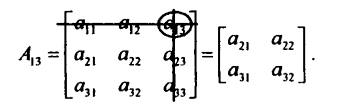
\includegraphics[max width=\textwidth]{matrix45}

Abbreviating the determinant of the matrix $A$ by $\operatorname{det}(A)$, the determinant of the $3 \times 3$ matrix $A$ is given by the following formula:
$$
\operatorname{det}(A)=a_{11} \operatorname{det}\left(A_{11}\right)-a_{12} \operatorname{det}\left(A_{12}\right)+a_{13} \operatorname{det}\left(A_{13}\right) .
$$
Since we have already shown how to compute the determinant of a $2 \times 2$ matrix, the right side can be thus computed. For a general $n \times n$ matrix $A$, we can compute it with a similar formula in terms of some of its $(n-1) \times(n-1)$ submatrices:

Below are two MATLAB commands that are used to work with entries and submatrices of a given general matrix $A$.
\\

$
\begin{array}{|l|l|}
\hline \begin{array}{l}
\text {A(i,j )} \rightarrow
\end{array} & \begin{array}{l}
\text {Represents the entry $a_{ij}$ located in the ith row and the } \\
\text{jth column of the matrix A.}
\end{array} \\
\hline \begin{array}{l}
\text {A([i1 i2 ... imax])}\\
\text {A([ji j2 ... jmax])}\rightarrow
\end{array} & \begin{array}{l}
\text {Represents the submatrix of the matrix $A$ formed using the } \\
\text{rows $i1, i2,..., imax$ and columns $j1,j2, ...,jmax.$ }
\end{array} \\
\hline \begin{array}{l}
\text {A([i1 i2 ... imax] , :)} \rightarrow
\end{array} & \begin{array}{l}
\text {Represents the submatrix of the matrix $A$ formed using the } \\
\text{rows $i1, i2,..., imax$ and all columns}
\end{array} \\
\hline
\end{array}
$ \\

\textbf{EXAMPLE 4.9:} (a) Write a MATLAB function file, called mydet2 (A), that calculates the determinant of a $2 \times 2$ matrix $A$.

(b) Using your function mydet 2 of part (a), build a new MATLAB function file called mydet $3(A)$ that computes the determinant of a $3 \times 3$ matrix $A$ (by performing cofactor expansion along the first row).

(c) Write a program mydet (A) that will compute the determinant of a square matrix of any size. Test it on the matrices shown below. MATLAB has a built-in function det for computing determinants. Compare the results, flop counts (if available), and times using your function mydet versus MATLAB's program det. Perform this comparison also for a randomly generated $8 \times 8$ matrix. Use the following command to generate random matrices:\\

$
\begin{array}{|l|l|}
\hline \begin{array}{l}
\text {rand(n,m)} \rightarrow \\
\text{NOTE: rand (n) is equivalent to} \\
\text{rand (n, n), and rand to rand (1).}\\
\end{array} & \begin{array}{l}
\text {Generates an $ n \times m$ w matrix whos entries are}\\
\text{randomly selected from 0 \footnote[5]{ Actually, the rand function, like any computer algorithm, uses a deterministic program to generate
random numbers that is based on a certain seed number (starting value). The numbers generated meet
statistical standards for being truly random, but there is a serious drawback that at each fresh start of a
MATLAB session, the sequence of numbers generated by successive applications of rand will always result in the same sequence. This problem can be corrected by entering
$rand( state' , sum(100*clock))$, which resets the seed number in a somewhat random
fashion based on the computer's internal clock. This is useful for creating simulation trials. } }
\end{array} \\
\hline
\end{array}
$ \\

SOLUTION: The programs in parts (a) and (b) are quite straightforward: 

\begin{verbatim}
function y = mydet2(A)
y=A(1,1)*A(2,2)-A(1,2)*A(2,1);
function y = mydet3(A)
y=A(1,1)*mydet2(A(2:3,2:3))-A(1,2)*mydet2(A(2:3,[1...
3]))+A(1,3)*mydet2(A(2:3,1:2)); 

\end{verbatim}

NOTE: The three dots $(\ldots)$ at the end of a line within the second function indicate (in MATLAB) a continuation of the command. This prevents the carriage return from executing a command that did not fit on a single line.

The program for part (c) is not quite so obvious. The reader is strongly urged to try and write one now before reading on.

Without having the mydet program call on itself, the code would have to be an extremely inelegant and long jumble. Since MATLAB allows its functions to (recursively) call on themselves, the program can be elegantly accomplished as follows:

\begin{verbatim}
function y = mydet(A)
y=0; %initialize y
[n, n] = size(A); %record the size of the square matrix A
if n ==2
y=mydet2(A) ;
return
end
for i=l:n
y=y+(-1)-^(i + 1)*A(1,i)*mydet(A(2:n, [1:(i-1) (i+1):n]));
end 
\end{verbatim}

Let's now run this program side by side with MATLAB's det to compute the requested determinants.

\begin{verbatim}
>>A=[2 7 8 10; 0 -1 4 -9 ; 0 0 3 6; 0 0 0 5] ;
>> A1=[1 2 -1 -2 1 2;0 3 0 2 0 1;1 0 2 0 3 0;1 1 1 1 1 1; . . .
-2-10123 ; 123123] ;

>>flops(0) , tic , mydet(A), toc , flops
->ans = -30(=determinant), elapsed_time = 0.0600, ans = 182 (=flop count)

>> flops(0) , tic , mydet(Al), toc , flops
->ans = 324, elapsed_time = 0.1600, ans =5226

>> flops(0) , tic , det(A), toc , flop s
->ans =-30, elapsedjime = 0, ans =52

>> flops(0) , tic , det(Al) , toc , flops
->ans =324, elapsed_time = 0, ans = 117
\end{verbatim}

So far we can see that MATLAB's built-in $det$ works quicker and with a lot less
flops than our mydet does. Although $mydet$ still performs reasonably well, check out the flop-count ratios and how they increased as we went from the $4 \times 4$ matrix $A$ to the $6 \times 6$ matrix $A 1$. The ratio of flops mydet used to the number that det used rose from about a factor of $3.5$ to a factor of nearly 50 . For larger matrices, the situation quickly gets even more extreme and it becomes no longer practical to use mydet. This is evidenced by our next computation with an $8 \times 8$ matrix.\\

\begin{verbatim}
>>Atest = rand(8) ; %we suppress outpu t here .
>>flops(0) , tic , det(Atest) , toc , flops
->ans = -0.0033, elapsedjime = 0, ans = 326 
>> flops(0) , tic , mydet(Atest) , toc , flops
->ans = -0.0033, elapsedjime =8.8400, ans = 292178 
\end{verbatim}

MATLAB's det still works with lightning speed (elapsed time was still undetectable) but now mydet took a molasses-slow nearly 9 seconds, and the ratio of the flop count went up to nearly 900 ! If we were to go to a $20 \times 20$ matrix, at this pace, our mydet would take over 24 years to do! (See Exercise 5 below.) Suprisingly though, MATLAB's det can find the determinant of such a matrix in less than $1 / 100$ of a second (on the author's computer) with a flop count of only about 5000 . This shows that there are more practical ways of computing (large matrix determinants) than by the definition or by cofactor expansion. In Chapter 7 such a method will be presented.

Each time when the rand command is invoked, MATLAB uses a program to generate a random numbers so that in any given MATLAB session, the sequence of "random numbers" generated will always be the same. Random numbers are crucial in the important subject of simulation, where trials of certain events that depend on chance (like flipping a coin) need to be tested. In order to assure that the random sequences are different at each start of a MATLAB session, the following command should be issued before starting to use rand:\\

$
\begin{array}{|l|l|}
\hline \begin{array}{l}
\text {rand('state',sum(100*clock))}\\
\rightarrow
\end{array} & \begin{array}{l}
\text {This sets the "state" of MATLAB's random } \\
\text {number generator in a way that}\\
\text {depends in a complicated fashion on the} \\
\text {current computer time. It will be different}\\
\text { each time MATLAB is started.} 
\end{array} \\
\hline
\end{array}
$ \\

Our next exercise for the reader will require the ability to store strings of text into rows of numerical matrices, and then later retrieve them. The following basic example will illustrate how such data transformations can be accomplished: We first create text string $\mathrm{T}$ and a numerical vector $\mathrm{v}$ :

\begin{verbatim}
>> T = 'Test' , v = [1 2 3 4 5 6]
->T = Test, v= 1 2 3 4 5 6 

\end{verbatim}

If we examine how MATLAB has stored each of these two objects, we learn that both are "arrays," but $T$ is a "character array" and $v$ is a "double array" (meaning a matrix of numbers):
\begin{verbatim}>> whos T v \end{verbatim}
\noindent \begin{tabular}{cccc}
->Name  &Size  &Bytes & Class  \\
T & 1x4 & 8 & char array\\
v & 1x6 & 48 & double char
\end{tabular}

If we redefine the first four entries of the vector $v$ to be the vector $T$, we will see that the characters in $\mathrm{T}$ get transformed into numbers:\\

\begin{verbatim}
» v(1:4)=T
->v = 84 101 115 116 5 6 
\end{verbatim}\\

MATLAB does this with an internal dictionary that translates all letters, numbers, and symbols on the keyboard into integers (between 1 and 256, in a case-sensitive fashion). To transform back to the original characters, we use the char command, as follows:\\

\begin{verbatim}
>> U=char(v(1:4))
->U =Test 
\end{verbatim}

Finally, to call on a stored character (string) array within an $fprint f$ statement, the symbol \%s is used as below:

\begin{verbatim}
» fprintf('Th e %s has been performed.' , Ü)
->The Test has been performed. 
\end{verbatim}

EXERCISE FOR THE READER 4.4: (\emph{Electronic Raffle Drawing Program})

(a) Create a script M-file, $raffledraw$, that will randomly choose the winner of a raffle as follows: When run, the first thing the program will do is prompt the user to enter the number of players (this can be any positive integer). Next it will successively ask the user to input the names of the players (in single quotes, as text strings are usually inputted) along with the corresponding weight of each player. The weight of a player can be any positive integer and corresponds to the number of raffle tickets that the player is holding. Then the program will randomly select one of these tickets as the winner and output a phrase indicating the name of the winner.

(b) Run your M-file with the following data on four players: Alfredo has four tickets, Denise has two tickets, Sylvester has two tickets, and Laurie has four tickets. Run it again with the same data.\\

\hrule width \hsize \kern 1pt \hrule width \hsize height 0.4pt

\hspace{0.1cm}

\textbf{EXERCISES 4.3: }
\begin{enumerate}
\item Write a MATLAB function M-file, call it sum $3 \mathrm{sq}(\mathrm{n})$, that takes as input a positive integer $n$ and as output will do the following. If $n$ can be expressed as a sum of three squares (of positive integers), i.e., if the equation:\\

$$
n=a^{2}+b^{2}+c^{2}
$$
has a solution with $a, b, c$ all positive integers, then the program should output the sentence, "The number $\langle n\rangle$ can be written as the sum of the squares of the three positive integers $\langle a\rangle$, $\langle b\rangle$, and $\langle c\rangle$." Each of the numbers in brackets must be actual integers that solve the equation. In case the equation has no solution (for $a, b, c$ ), the output should be the sentence: "The number $\langle n\rangle$ cannot be expressed as a sum of the squares of three positive integers." Run your program with the numbers $n=3, n=7, n=43, n=167, n=994, n=2783, n=25,261$. Do you see a pattem for those integers $n$ for which the equation does/does not have a solution? 
\item Repeat Exercise 1 with "three squares" being replaced by "four squares," so the equation becomes:
$$
n=a^{2}+b^{2}+c^{2}+d^{2}
$$
Call your function sum 4 sq. In each of these problems feel free to run your programs for a larger set of inputs so as to better understand any patterns that you may perceive.

\item (\emph{Number Theory: Perfect Numbers}) (a) Write a MATLAB function M-file, call it divsum (n), that takes as input a positive integer $\mathrm{n}$ and gives as output the sum of all of the proper divisors of $\boldsymbol{n}$. For example, the proper divisors of 10 are 1,2 , and 5 so the output of divsum (10) should be $8(=1+2+5)$. Similarly, divsum $(6)$ should equal 6 since the proper divisors of 6 are 1,2 , and 3. Run your program for the following values of $n: n=10, n=224, n=1410$ (and give the outputs).

(b) In number theory, a perfect number is a positive integer $n$ that equals the sum of its proper divisors, i.e., $n=\operatorname{divsum}(n)$. Thus from above we see that 6 is a perfect number but 10 is not. In ancient times perfect numbers were thought to carry special magical properties. Write a program that uses your function in part (a) to get MATLAB to find and print all of the perfect numbers that are less than 1000 . Many questions about perfect numbers still remain perfect mysteries even today. For example, it is not known if the list of perfect numbers goes on forever.

\item (\emph{Number Theory: Prime Numbers}) Recall that a positive integer $n$ is called a prime number if the only positive integers that divide evenly into $n$ are 1 and itself. Thus 4 is not a prime since it factors as $2 \times 2$. The first few primes are as follows: $2,3,5,7,11,13,17,19,23, \ldots(1$ is not considered a prime for some technical reasons). There has been a tremendous amount of research done on primes, and there still remain many unanswered questions about them that are the subject of contemporary research. One of the first questions that comes up about primes is whether there are infinitely many of them (i.e., does our list go on forever?). This was answered by an ancient Greek mathematician, Euclid, who proved that there are infinitely many primes. It is a very time-consuming task to determine if a given (large) number is prime or not (unless it is even or ends in 5).

(a) Write a MATLAB function M-file, call it primeck ( $n)$, that will input a positive integer $n$ $>1$, and will output either the statement: "the number $\langle n\rangle$ is prime," if indeed, $n$ is prime, or the statement "the number $\langle n\rangle$ is not prime, its smallest prime factor is $<k>$," if $n$ is not prime, and here $k$ will be the actual smallest prime factor of $n$.

Test (and debug) your program for effectiveness with the following inputs for $n$ :
$$
n=51, n=53, n=827, n=829 .
$$
Next test your program for efficiency with the following inputs (depending on how you wrote your program and also how much memory your computer has, it may take a very long time or not finish with these tasks)
$$
\begin{aligned}
n=8237, n=38877, n &=92173, n=1,875,247, n=2038074747, n=22801763489, \\
n &=1689243484681, n=7563374525281 .
\end{aligned}
$$
In your solution, make sure to give exactly what the MATLAB printout was; also, next to each of these larger numbers, write down how much time it took MATLAB to perform the calculation.

(b) Given enough time (and assuming you are working on a computer that will not run out of memory) will this MATLAB program always work correctly no matter how large $n$ is? Recall that MATLAB has an accuracy of about 15 significant digits.

\item We saw in Example $4.7$ that by calculating a determinant by using cofactor expansion, the number of flops (additions, subtractions, multiplications, and divisions) increases dramatically. For a $2 \times 2$ matrix, the number (worst-case scenario, assuming no zero entries) is 3 ; for a $3 \times 3$ matrix it is 14. What would this number be for a $5 \times 5$ matrix?, For a $9 \times 9$ matrix? Can you determine a general formula for an $n \times n$ matrix?

 \item (\emph{Probability and Statistics}) Write a program called cointoss ( $n$ ) that will have one input variable $n=$ a positive integer and will simulate $\mathrm{n}$ coin tosses, by (internally) generating a sequence of $n$ random numbers (in the range $0 \leq x \leq 1$ ) and will count each such number that is less than $0.5$ as a "HEAD" and each such number that is greater than $0.5$ as a "TAIL." If a number in the generated sequence turns out to be exactly $=0.5$, another simulated coin toss should be made (perhaps repeatedly) until a "HEAD" or a "TAlL" comes up. There will be only one output variable: $P=$ the ratio of the total number of "HEADS" divided by $n$. But the program should also cause the following sentence to be printed: "In a trial of $<n>$ coin tosses, we had $<\mathrm{H}>$ flips resulting in 'HEAD' and $\angle \mathrm{T}>$ flips resulting in 'TAlL,' so 'HEADS' came up $<100 \mathrm{P}>\%$ of the time." Here, $<\mathrm{H}>$ and $<\mathrm{T}>$ are to denote the actual numbers of "HEAD" and "TAlL" results. Run your program for the following values of $n: 2,4,6,10,50,100,1000$, $5000,50,000$. Is it possible for this program to enter into an infinite loop? Explain!

\item (\emph{Probability and Slatistics}) Write a program similar to the one in the previous exercise except that it will not print the sentence, and it will have three output variables: $P$ (as before), $H=$ the number of heads, and $T=$ the number of tails. Set up a loop to run this program with $n=1000$ fixed for $k=100$ times. Collect the outcomes of the variable $H$ as a vector: $\left[h_{0}, h_{1}, h_{2}, \cdots h_{n+1}\right]$ (with $n+1=1001$ entries) where each $h$, denotes the number of times that the experiment resulted in having exactly $h_{i}$ heads (so $H=h_{i}$ ) and then plot the graph of this vector (on the $x$-axis $n$ runs from 0 to 1001 and on the $y$-axis we have the $h_{i}$-values). Repeat this exercise for $k=200$ and then $k=500$ times.

\item (\emph{Probability: Random Integers}) Write a MATLAB function M-file, randint $(\mathrm{n}, \mathrm{k})$, that has two input variables $\mathrm{n}$ and $\mathrm{k}$ being positive integers. There will be one output variable $R, a$ vector with $k$ components $R=\left[r_{1}, r_{2}, \cdots, r_{k}\right]$, each of whose entries is a positive integer randomly selected from the list $\{1,2, \ldots, n\}$. (Each integer in this list has an equal chance of being generated at any time.)

\item (\emph{Probability: Random Walks}) Create a MATLAB M-file called ran2walk (n) that simulates a random walk in the plane. The input $n$ is the number of steps in the walk. The starting point of the walk is at the origin $(0,0)$. At each step, random numbers are chosen (with uniform distribution) in the interval $[-1 / 2,1 / 2]$ and are added to the present $x$ - and $y$-coordinates to get the next $x$ - and $y$-coordinates. The MATLAB command rand generates a random number in the interval $[0,1]$, so we must subtract $0.5$ from these to get the desired distributions. There will be no output variables, but MATLAB will produce a plot of the generated random walk.

Run this function for the values $n=8,25,75,250$ and (using the subplot option) put them all into a single figure. Repeat once again with the same values. In three dimensions, these random walks simulate the chaotic motion of a dust particle that makes many microscopic collisions and produces such strange motions. This is because the microscopic particles that collide with our particle are also in constant motion. We could easily modify our program by adding a third $z$-coordinate (and using plot $3(x, y, z)$ instead of plot $(x, y))$ to make a program to simulate such three-dimensional random walks. Interestingly, each time you run the ran2walk function for a fixed value of $n$, the paths will be different. Try it out a few times. Do you notice any sort of qualitative properties about this motion? What are the chances (for a fixed $n$ ) that the path generated will cross itself? How about in three dimensions? Does the motion tend to move the particle away from where it started as $n$ gets large? For these latter questions do not worry about proofs, but try to do enough experiments to lead you to make some educated hypotheses.

\item(\emph{Probability Estimates by Simulation}) In each part, run a large number of simulations of the following experiments and take averages to estimate the indicated quantities.

(a) Continue to generate random numbers in $(0,1)$ using rand until the accumulated sum exceeds 1 . Let $N$ denote the number of such random numbers that get added up when this sum first exceeds 1. Estimate the expected value of $N$, which can be thought of as the theoretical (long-run) average value of $N$ if the experiment gets repeated indefinitely.

(b) Number a set of cards from 1 to 20, and shuffle them. Tum the cards over one by one and record the number of times $K$ that card number i $(1 \leq i \leq 20)$ occurs at (exactly) the $i$ th draw. Estimate the expected value of $K$.

Note: Simulation is a very useful tool for obtaining estimates for quantities that can be impossible to estimate analytically; see [Ros-02] for a well-written introduction to this interesting subject. In it the reader can also find a rigorous definition of the expectation of a random variable associated with a (random) experiment. The quantities $K$ and $N$ above are examples of random variables. Their outcomes are numerical quantities associated with the outcomes of (random) experiments. Although the outcomes of random variables are somewhat unpredictable, their long-term averages do exhibit patterns that can be nicely characterized.

For the above two problems, the exact expectations are obtainable using methods of probability; they are $N=e$ and $K=1$.

The next four exercises will revisit the Collatz conjecture that was introduced in the preceding section.

\item (Number Theory: The Collatz Problem) Write a function M-file, call it collsz, that takes as input a positive integer an (the first element for a Collatz experiment), and has as output a positive integer size equaling the size of the largest number in the Collatz iteration sequence before it reaches the value of 1 . What is the first positive integer an for which this maximum size exceeds the value 100 ? 1000 ? 100,000 ? 1,000,000?

  \item (Number Theory: The Collatz Problem) Modify the script file, col1at , of Example 4.7 in the text to a new one, collatzg, that will interactively take the same input and intemally construct the same vector a, but instead of producing output on the command window, it should produce a graphic of the vector a's values versus the index of the vector. Arrange the plot to be done using blue pentagrams connected with lines. Run the script using the following inputs: 7 , 15,27,137,444,657.

Note: The syntax for this plot style would be \begin{verbatim}plot (index, a, bp-).\end{verbatim}

\item (Number Theory: The Collatz Problem) If a Collatz experiment is started using a negative integer for $a(1)$, all experiments so far done by researchers have shown that the sequence will eventually cycle. However, in this case, there is more than one possible cycle. Write a script, $collatz2$, that will take an input for $a(1)$ in the same way as the script collatz in Example 4.7 did, and the script will continue to do the Collatz iteration until it detects a cycle. The output should include the number of iterations done before detecting a cycle as well as the actual cycle vector. Run your script using the following inputs: $-2,-4,-8,-10,-56,-88, -129$.

Suggestion: A cycle can be detected as soon as the same number $a(n)$ has appeared previously in the sequence. So your script will need to store the whole Collatz sequence. For example, each time it has constructed a new sequence element, say $a(20)$, the script should compare with the previous vector elements $a(1), a(20), \ldots, a(19)$ to see if this new element has previously appeared. If not, the iteration goes on, but if there is a duplication, say, $a(20)=a(15)$, then there will be a cycle and the cycle vector would be $(a(15), a(16), a(17), a(18), a(19))$

\item (Number Theory: The Collatz Problem) Read first the preceding exercise. We consider two cycles as equivalent in a Collatz experiment if they contain the same numbers (but not necessarily in the same order). Thus the cycle $(1,4,2)$ has the equivalent forms $(4,2,1)$, and $(2,1,4)$. The program in the previous exercise, if encountering a certain cycle, may output any of the possible equivalent forms, depending on the first duplication encountered. We say that two cycles are essentially different if they are not equivalent cycles. In this exercise, you are to use MATLAB to help you figure out the number of essentially different Collatz cycles that come up from using negative integers for $a(1)$ ranging from $-1$ to $-20,000$.

Note: The Collatz conjecture can be paraphrased as saying that all Collatz iterations starting with a positive integer must eventually cycle and the resulting cycles are all equivalent to $(4,2,1)$. The essentially different Collatz cycles for negative integer inputs in this problem will cover all that are known to this date. It is also conjectured that there are no more.
\end{enumerate}

\end{document}